% The Finite Element Method

\vskip -0.2in % Make space for first page text...
\section{Introduction}

Continuum mechanics provides the foundation for understanding of fluid motion, and the Navier-Stokes equations for
a Newtonian fluid are the primary model for the prediction of fluid behaviour in engineering.
The domain and initial/boundary conditions can be arbitrarily complex. For example, fluid motion is often simulated
through a digital surface model of a real-world object or system created in computer-aided design software.
On the other side of the coin, fluid models are very often used in modern film, both live action and animated.
\captionsetup[subfigure]{labelformat=empty}
\begin{figure}[H]
    \centering
    \subfloat[][\centering Peter Dirichlet (1805--1859)]{{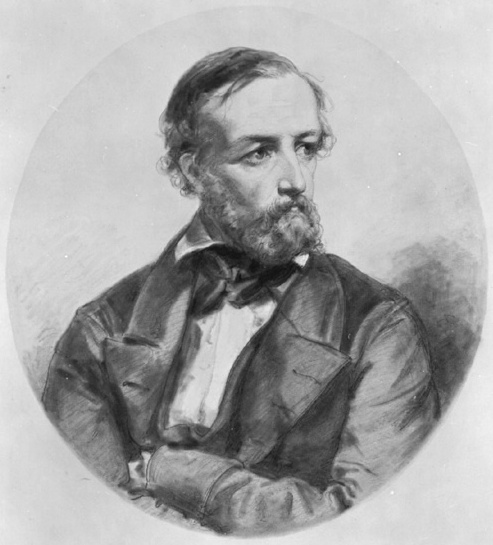
\includegraphics[height=2.9cm]{figures/mathematicians/Peter_Dirichlet.jpg} }}
    \qquad
    \subfloat[][\centering David Hilbert (1862--1943)]{{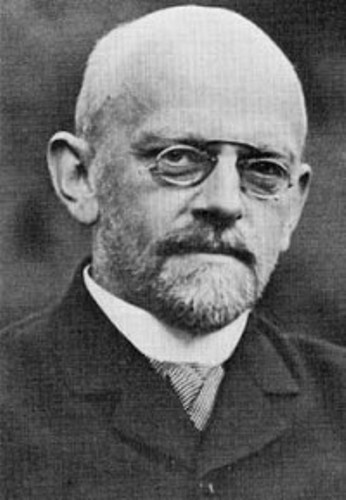
\includegraphics[height=2.9cm]{figures/mathematicians/David_Hilbert.jpeg} }}
    \qquad
    \subfloat[][\centering Walther Ritz (1878--1909)]{{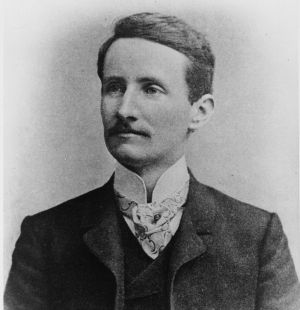
\includegraphics[height=2.9cm]{figures/mathematicians/Walther_Ritz.jpg} }}
    \qquad
    \subfloat[][\centering Boris Galerkin (1871--1945)]{{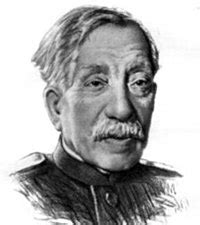
\includegraphics[height=2.9cm]{figures/mathematicians/Boris_Galerkin.jpeg} }}
    \qquad
    \subfloat[][\centering Sergei Sobolev (1908--1989)]{{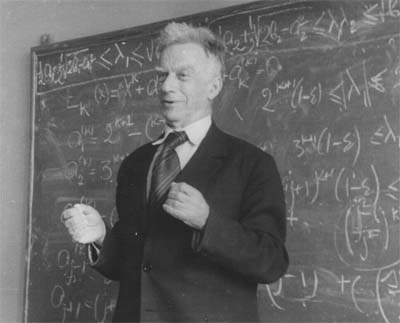
\includegraphics[height=3.4cm]{figures/mathematicians/Sergei_Sobolev.jpg} }}
    \qquad
    \subfloat[][\centering Laurent Schwartz (1915--2002)]{{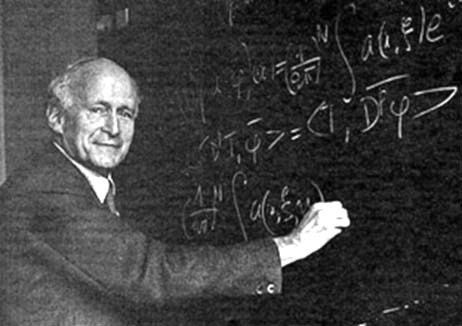
\includegraphics[height=3.4cm]{figures/mathematicians/Laurent_Schwartz.jpeg} }}
    \caption{Some key figures whose work precipitated modern developments in PDEs.}
    \label{fig:galerkin_mathematicians}
\end{figure}
In applications, the Navier-Stokes equations are primarily
solved on a computer, and a computer works with both finite data and finite precision. The Galerkin method
is particularly amenable to computer implementation, so much so that the whole process of geometric modelling, boundary condition handling,
residual minimisation, and solution reconstruction, can be automated (\cite{firedrake}, \cite{fenics_book}, \cite{DOLFIN}). We begin by
deriving two instances of Galerkin methods for Poisson's equation, performed on an irregular 2D domain to emphasize that the methods trivially extend
to complex geometries. A computer implementation is then presented, which generates visualisations and quality metrics for the results.



\subsubsection{The Galerkin method}
The Galerkin method was established by engineer and mathematician Boris Galerkin (1871--1945) in a 1915 paper containing
an approximation method for the biharmonic equation of classical beam theory \cite{boris_galerkin}. Briefly, the principle of Galerkin is to
choose a space of approximations, today called ``test functions'', and solve for the test function which minimises a residual error with respect
to some function space norm. This norm is induced by a choice of what are now called the ``trial functions''. If the trial functions are the same as the test functions,
the residual is minimised with respect to the Euclidean norm.

As well as proving highly useful
in numerical applications, the methods of Galerkin (and preceding work by mathematicians such as Walther Ritz) proved important to further developments
in the mathematical theory of PDEs. In a 1934 talk named ``Generalized Solutions to the Wave Equation'', mathematician Sergei L. Sobolev (1908--1989)
precipitated the development
of generalised functions by Laurent Schwartz (1915-2002), integral to the modern study of PDEs
(\cite{sobolev_web_page}, \cite{one_hundred_years_galerkin}).
These developments are clarifications on the question: What do we mean when we speak of a solution to a PDE from physics? Galerkin's method
is much closer to the answer than, for example, the finite difference method.


\subsubsection{The finite element method}

\section{The equation to solve: The Poisson equation}

Among the fundamental PDEs
are the heat equation
    $$\Part{h}{t} = \Delta h + g$$
and Poisson's equation
\begin{equation}\label{poisson_compact}
    -\Delta h = g.
\end{equation}
The latter can be thought of as the steady-state version of the former. The solution of a Poisson problem will be a crucial component
of the solution of the Stokes equations. It seems ideal to start by discussing
discretization methods for Poisson's equation \eqref{poisson_compact} in particular,
as it is likely the simplest non-trivial PDE.
The focus here is on the Dirichlet problem
\begin{equation}\label{poisson_dirichlet_problem}
    -\Delta h = g, \quad \left.h\right|_{\Gamma} = h_\Gamma,
\end{equation}
where $\Gamma$ is the boundary of the domain, and the domain is 2D.

\subsection{Discretizing the differential form of the PDE}
It is a theorem of Gauss that in Euclidean space $\mathbb{R}^3$ we have
\begin{equation}\label{gauss_euclidean_divergence}
    \nabla \cdot v = \Part{v_x}{x} + \Part{v_y}{y} + \Part{v_z}{z},
\end{equation}
and we get \eqref{poisson_compact} in the form
\begin{equation}\label{poisson_differential_intro}
    -\left(\frac{\partial^2 h}{\partial x^2}
           +\frac{\partial^2 h}{\partial y^2}
           +\frac{\partial^2 h}{\partial z^2}\right) = g.
\end{equation}
Thinking about \eqref{poisson_differential_intro} leads to the finite difference method, historically the first and
still very important in applications.
By forming secant approximations of the derivatives over a regular grid, a linear system is formed, and the approximate solution is solved
for as a function of this grid.
However, it may be hard to give a real interpretation of what the solution samples at grid points say about the solution everywhere.
They could be coefficients of, for example, hat basis functions.
Yet a finite difference discretization of Poisson equation \eqref{poisson_compact} may not take this into account at all. One might feel that
limits have been taken too soon.

% Consider a single conservation law as described in section \ref{conservation_laws}. This law
% was given in two forms, ``integral'' \eqref{continuity_equation}:
% \begin{equation*}
%     \frac{d}{dt} \int_{\Omega_0} \phi\,dx = \int_{\Omega_0} s\,dx + \int_{\pomn} \phi j \cdot \left(-\hat{n}\right)\,dx,
% \end{equation*}
% and ``differential'' \eqref{continuity_equation_differential}:
% \begin{equation*}
%     \Part{\phi}{t} = s - \nabla\cdot (\phi j).
% \end{equation*}

\subsection{Discretizing the integral form of the PDE}
In physics, Poisson's equation is an equilibrium conservation law, and therefore has an integral form.
This form will give clearer routes to discretizations which
have geometric meaning.
% Thinking instead about \eqref{poisson_integral_intro} will lead to Galerkin methods, which include finite volumes, finite elements, and spectral methods.
For example, the general integral conservation law \eqref{continuity_equation},
\begin{align*}
    \frac{d}{dt} \int_{\Omega_0} \phi\,dx = \int_{\Omega_0} s\,dx + \int_{\pomn} \phi j \cdot \left(-\hat{n}\right)\,dx,
\end{align*}
is a geometric statement about fluxes
of quantity $\phi$ by $j$, quantified over arbitrary control volumes $\Omega_0$.
There are an infinite number of control volumes, and therefore an infinite number of equations which must hold, and there is an infinite dimensional
space of solutions to choose from. A key idea, then, is to choose a finite number of equations and a finite dimensional subspace of possible approximate solutions.
A supposed solution will be represented by the coefficients of some choice of basis functions for the subspace. Each equation will be checked exactly against this supposed solution.
To continue with this idea, we must write Poisson's equation \eqref{poisson_compact} in integral form.

% \vskip 0.2in
% (figure)
% \vskip 0.2in
% 
% Finite element methods, and more generally Galerkin methods, live comfortably in the language of weak solutions, integral forms of partial differential equations,
% and the calculus of variations.
% To continue with this idea, we must write Poisson's equation \eqref{poisson_compact} in integral form.

\subsubsection{Deriving the heat and Poisson equation through diffusion processes}
The Poisson equation \eqref{poisson_compact} can be thought of as the steady state of some diffusion process with a source term $g$,
although this need not be its literal physical interpretation.
A diffusion process ``levels out'' some quantity, such as temperature or some chemical concentration.
A diffusion could intuitively be thought of as a
progressive ``blurring'',
such as in a camera defocus, and in fact many common image processing techniques use diffusion PDEs from physics \cite{tum}. We will stick with
the notion of ``temperature'' $h$ as the diffused quantity.
\textit{Fick's law of diffusion} is a constitutive relation giving the bulk flux of temperature $h$ as proportional to the negative gradient:
    $$hj = -\mu\nabla h,$$
where $\mu$ is called the diffusion coefficient.
This is one way of saying that the temperature tends to level out.
If we form a continuity equation \eqref{continuity_equation} for temperature, with source $s$, we get
\begin{equation}\label{heat_equation_integral}
    \frac{d}{dt} \int_{\Omega_0} h\,dx = \int_{\Omega_0} s\,dx + \int_{\pomn} \mu \nabla h \cdot \hat{n}\,dx,
\end{equation}
which by application of Stokes' theorem becomes
\begin{equation}\label{heat_equation_differential}
    \frac{dh}{dt} = s + \nabla \cdot \left(\mu \nabla h\right).
\end{equation}
If we further assume that the diffusion coefficient $\mu$ is constant, we get
\begin{equation}\label{heat_equation_differential_constant}
    \frac{dh}{dt} = s + \mu\nabla \cdot \nabla h = s + \mu\Delta h,
\end{equation}
which is the standard heat equation.
The steady-state heat equation is then
\begin{equation}\label{poisson_equation}
    -\Delta h = g,
\end{equation}
where we let $g = s/\mu$ in the above.
This completes the derivation of Poisson's equation \eqref{poisson_compact}.
% which models steady-state diffusion processes and can be used to calculate gravitational or electrostatic potential fields.
In integral form, ``undoing'' the application of Stokes' theorem above, Poisson's equation is
\begin{equation}\label{poisson_equation_integral}
    \int_{\pomn} -\nabla h\cdot \hat{n}\,dx = \int_{\omn} g\,dx \quad \text{for all control volumes $\Omega_0$.}
\end{equation}
Form \eqref{poisson_equation_integral} clearly shows that we are calculating a steady state,
as we are solving for $h$ such that the amount of heat that leaves $\Omega_0$ is the amount introduced into $\Omega_0$ by the source function.
The form \eqref{poisson_equation_integral}, rather than \eqref{poisson_compact}, will be the starting point for deriving Galerkin methods.

\subsubsection{So how do we discretize Poisson's equation?}
Even starting with \eqref{poisson_equation_integral}, there are many routes to take to discretization.
Notice that there are two variables in \eqref{poisson_equation_integral}, although one is bound over universal quantification:
the control volume $\Omega_0$ and the function $h$.
The general Galerkin method very naturally appears when the ``space'' $\Omega_0$ resides in and the space $h$ resides in are reduced
such that the equations are both finite dimensional and well-determined. Firstly, let's derive the conceptually simplest
discretization method of these spaces, the finite volume method.


\section{Discretizing Poisson's equation by finite volumes}\label{discretizing_poisson}
---NOTE: $H^1$ May be wrong.
---NOTE: Should discuss interpretation in terms of residual minimisation with respect to some norm.

Equation \eqref{poisson_equation_integral} is quantified over an infinite number of control volumes $\Omega_0$.
These control volumes are in the interior of $\Omega$, as the solution at the boundary $\Gamma$ is specified by the Dirichlet boundary condition
$\left.h\right|_\Gamma = h_\Gamma$, and there is no flux information across $\Gamma$.
A simple idea is to choose a finite number of control volumes $\Omega_1,\cdots,\Omega_n$ (hence ``finite volumes''), and check that the flux integral holds over each of these.
We will then have $n$ equations on $h$. As this system will be underdetermined ($h$ has infinite degrees of freedom), we must
restrict $h$ to a finite dimensional space of approximations $\Phi^*$.

We begin by discussing the general construction of a finite volume method, but this will soon be made concrete with a simple, specific example of a 
finite volume discretization.


\subsection{The Dirichlet boundary condition and the test space}
The Dirichlet boundary condition $\left.h\right|_\Gamma = h_\Gamma$ specifies the boundary values for any solution.
However, the finite dimensional space $\Phi^*$ may not be able to exactly represent the boundary function $h_\Gamma$,
and therefore the first step is to approximate $h_\Gamma$ (for which there are many options, for example
projection in the $L^2$-norm or interpolation across a finite sampling of boundary points \cite{approximation_theory}). Choosing some $\phi_\Gamma \in \Phi^*$ with
    $$\left.\phi_\Gamma\right|_\Gamma \approx h_\Gamma,$$
we can define an ``interior'' function space
$$
    \Phi = \left\{h^* \in \Phi^* \mid \left.h\right|_\Gamma = 0 \right\},
$$
and the approximate solution $\tilde{h}$ will then be
$$
    \tilde{h} = \phi + \phi_\Gamma
$$
for some $\phi \in \Phi$.
In the finite volume and finite element literature the space $\Phi$ is called the test space.
Since we selected $n$ control volumes $\Omega_1,\cdots,\Omega_n$, the approximating space $\Phi^*$ must be chosen such that
$\Phi$ is $n$-dimensional. We can choose a basis for the test space,
    $$\Phi = \text{span}\left\{\phi_1,\cdots,\phi_n\right\}.$$
The problem is now to find a vector of coefficients of these test functions,
    $\hat{h} = (h_1, \cdots, h_n)^T,$
and reconstruct the solution as
    $$\tilde{h} = \phi + \phi_\Gamma,$$
where $\phi$ is the ``interior variation''
    $$\phi = \Phi\cdot \hat{h} \coloneqq h_1\phi_1 + \cdots + h_n\phi_n.$$

\subsection{Forming a linear system}
The integral-conservation-law form \eqref{poisson_equation_integral} of Poisson's equation \eqref{poisson_compact}
now directly indicates a method of approximation. Letting $h$ be approximated by $\tilde{h} = \phi + \phi_\Gamma$ (where $\phi \in \Phi$ is unknown and $\phi_\Gamma \in \Phi^*$ is known),
and restricting the flux integrals to the control volumes $\Omega_1,\cdots,\Omega_n$, the conservation law \eqref{poisson_equation_integral} becomes
\begin{equation}\label{poisson_equation_integral_fvm}
    \int_{\partial\Omega_j} -\nabla \left(\phi + \phi_\Gamma\right) \cdot \hat{n}\,dx = \int_{\Omega_j} g\,dx \quad\quad j=1,\cdots,n.
\end{equation}
The ``interior variation'' $\phi = \Phi\cdot \hat{h}$ is the only unknown, so we can move all knowns to the right-hand-side
and expand $\phi$ in terms of the basis test functions $\phi_1,\cdots,\phi_n$:
\begin{equation}\label{poisson_equation_integral_fvm_knowns_unknowns}
    \int_{\partial\Omega_j} -\nabla \left(\sum_{i=1}^nh_i\phi_i\right) \cdot \hat{n}\,dx =
            \int_{\Omega_j} g\,dx
            + \int_{\partial\Omega_j} \nabla \phi_\Gamma \cdot \hat{n}\,dx
 \quad\quad j=1,\cdots,n.
\end{equation}
By linearity, to emphasize the separate integrals that need to be computed, the above equation can be written as
\begin{equation}\label{poisson_equation_integral_discretized}
    \sum_{i=1}^n h_i\int_{\pom_j} -\nabla \phi_i \cdot \hat{n}\,dx =
            \int_{\Omega_j} g\,dx
            + \int_{\partial\Omega_j} \nabla \phi_\Gamma \cdot \hat{n}\,dx
 \quad\quad j=1,\cdots,n.
\end{equation}
It is seen here that there must be some restrictions on the $\phi_i$ and $\phi_\Gamma$.
Formally, they must be in the Sobolev space $H^1(\Omega)$
(--- NOTE: This is probably wrong, as the integrals are over internal cell boundaries and the boundary $\Gamma$. Need to read
about $H^{\text{div}}$)
This simply means that they must have a gradient defined ``almost everywhere''.
It does not matter if the gradient is not defined at isolated lower-dimensional subsets, as these make no contribution to
the integral. The system \eqref{poisson_equation_integral_discretized} can be written in matrix form as
\newcommand{\integralentry}[2]{\int_{\pom_{#1}}-\nabla\phi_{#2}\cdot\hat{n}\,dx}
\newcommand{\integralrhsentry}[1]{\int_{\om_{#1}}g\,dx + \int_{\pom_{#1}}\nabla\phi_\Gamma\cdot\hat{n}\,dx}
\begin{equation}\label{poisson_matrix_equation}
\begin{split}
    A\hat{h}
    &= \begin{bmatrix}
            \integralentry{1}{1} & \cdots & \integralentry{1}{n} \\
            \vdots & & \vdots \\
            \integralentry{n}{1} & \cdots & \integralentry{n}{n}
    \end{bmatrix}
    \begin{bmatrix} h_1 \\ \vdots \\ h_n \end{bmatrix}
    \\
    &= \begin{bmatrix} \integralrhsentry{1} \\ \vdots \\ \integralrhsentry{n}  \end{bmatrix}
    = \hat{f}.
\end{split}
\end{equation}
This system is solved for the coefficients of combination $\hat{h} = (h_1 \cdots h_n)^T$, and the approximate
solution is constructed as $\tilde{h} = \Phi\cdot\hat{h} + \phi_\Gamma$.
If the control volumes $\Omega_1,\cdots,\Omega_n$ and test space $\Phi = \text{span}\left\{\phi_1,\cdots,\phi_n\right\}$
are chosen well, this linear system will be nonsingular and hopefully well-conditioned.
If the chosen control volumes join together in the interior of $\Omega$ like pieces of a puzzle, this gives a conservative system of balanced fluxes, but it is another question whether the approximation
$\tilde{h}$ is good.

\newpage
% \subsection{Choosing the test space, boundary approximation, and control volumes}
\subsection{A piecewise linear triangulation scheme}
Possibly the simplest scheme is to triangulate $\Omega$ as
    $\bigcup_i T_i,$
such that there are $n$ interior vertices $p_1,\cdots,p_n$, and $n_\Gamma$ boundary vertices $p^\Gamma_1,\cdots,p^\Gamma_{n_\Gamma}$, and $n_T$ triangles
$T_1,\cdots,T_{n_T}$. An example triangulation of an ellipse-shaped domain is shown in figure \ref{triangulation}.
\begin{figure}[H]
    \begin{center}
        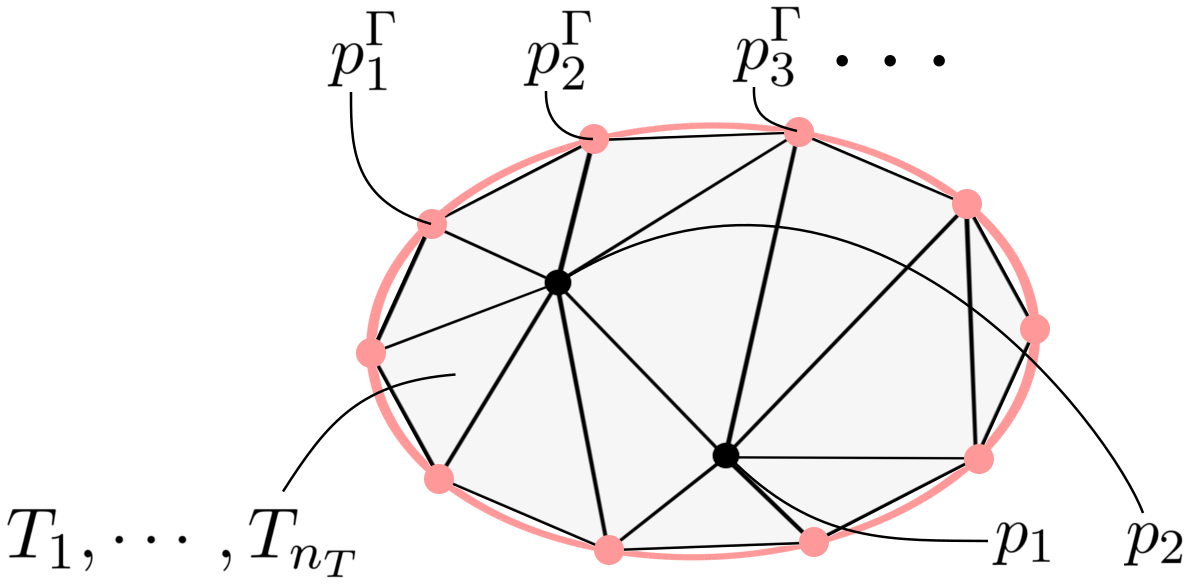
\includegraphics[width=0.53\linewidth]{figures/triangulation/triangulation.png}
    \end{center}
    \caption{\scriptsize
        The domain $\Omega$ is partitioned into $n_T = 12$ triangular cells $T_1\cdots T_{12}$. The boundary is sampled at $n_\Gamma = 10$ points
        $p^\Gamma_1,\cdots,p^\Gamma_{10}$.
        There are $n = 2$ interior points, $p_1$ and $p_2$.
    }
    \label{triangulation}
\end{figure}

\subsubsection{The test space}
Firstly, there is a clear choice of function space $\Phi^*$, which satisfies the $H^1$ condition
(NOTE: Is $H^1$ necessary? Need to check conditions for finite volumes), consisting of piecewise linear ``hat'' basis functions
at each interior or boundary vertex,
\newcommand{\hatfun}[1]{\text{Hat}(#1)}
$$
    \Phi^* = \text{span}\left\{
        \hatfun{p_1},\cdots,\hatfun{p_n},
        \hatfun{p^\Gamma_1},\cdots,\hatfun{p^\Gamma_{n_\Gamma}}
    \right\}.
$$
The hat function at a vertex has value $1$ at that vertex and value $0$ at its neighbours.
The test space (which is zero on the boundary $\Gamma$) is then
\begin{align*}
    \Phi &= \text{span}\left\{
        \hatfun{p_1},\cdots,\hatfun{p_n}
    \right\} = \text{span}\left\{\phi_1,\cdots,\phi_n\right\},
\end{align*}
where $\phi_i \coloneqq \text{Hat}(p_i)$.
One of these basis functions for the ellipse-shaped domain is shown in figure \ref{ellipse_partition}.
\begin{figure}[H]
    \begin{center}
        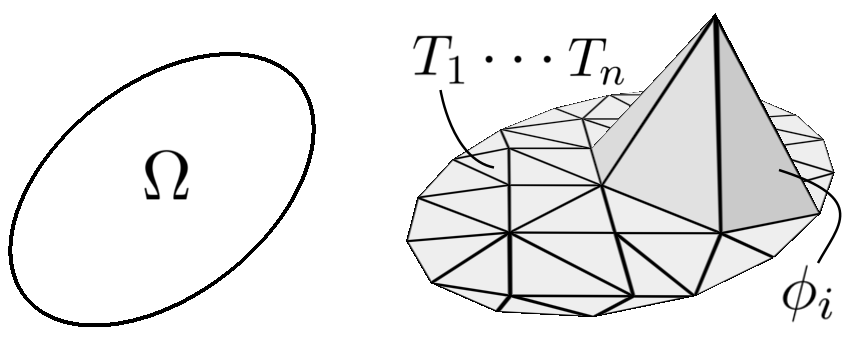
\includegraphics[width=0.53\linewidth]{figures/hat.png}
    \end{center}
    \caption{\scriptsize
        The domain $\Omega$ is partitioned into triangular cells $T_1\cdots T_{n_T}$. One example of a hat basis function $\phi_i$ is shown, where
        the vertical axis is the basis function value.
    }
    \label{ellipse_partition}
\end{figure}

\newpage
\subsubsection{Approximating the boundary values}
One simple approximation of $\left.h\right|_\Gamma = h_\Gamma$ is
$$
    \phi_\Gamma = h_\Gamma(p^\Gamma_1)\hatfun{p^\Gamma_1}
                + \cdots
                + h_\Gamma(p^\Gamma_{n_\Gamma})\hatfun{p^\Gamma_{n_\Gamma}},
$$
which is a piecewise linear interpolation when restricted to the boundary $\Gamma$. The approximation $\phi_\Gamma$ for some boundary
function $h_\Gamma$ is shown in figure \ref{boundary}.
\begin{figure}[H]
    \begin{center}
        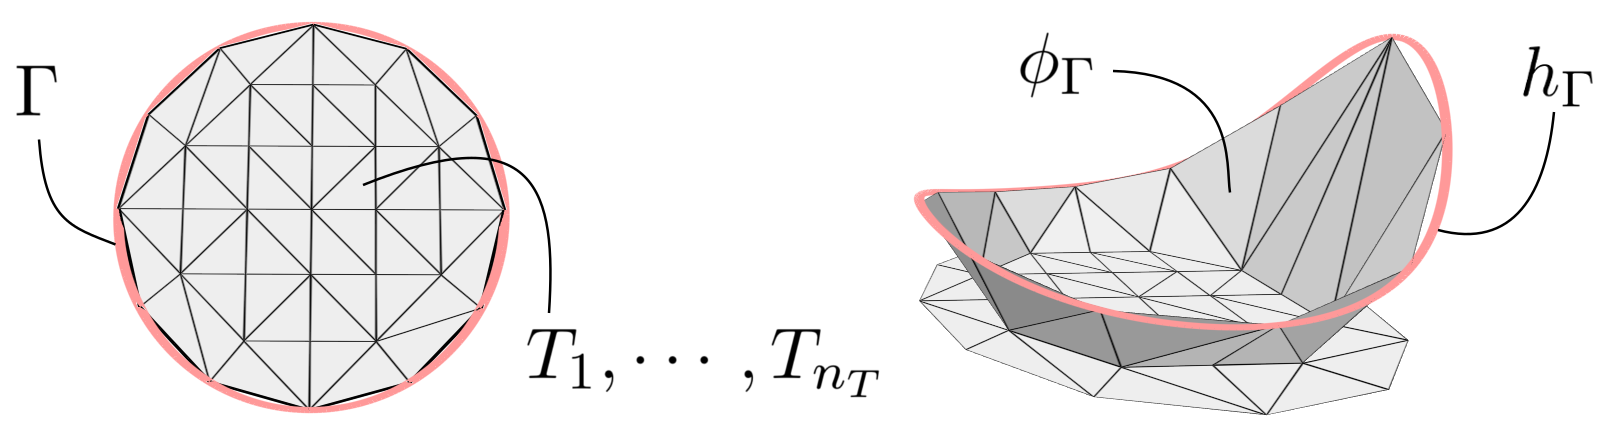
\includegraphics[width=0.9\linewidth]{figures/boundary/boundary.png}
    \end{center}
    \caption{\scriptsize
        A circle domain $\Omega$ with boundary $\Gamma$ is tessellated by triangles $T_1,\cdots,T_{n_T}$.
        The boundary function $h_\Gamma$ is approximated by $\phi_\Gamma$, a linear combination of hat functions centred at the boundary vertices.
    }
    \label{boundary}
\end{figure}
This approximation $\phi_\Gamma$ is added to the ``interior variation'' $\phi = \Phi\cdot\hat{h}$ to construct a possible solution.
When a linear solver is given the linear system \eqref{poisson_matrix_equation}, it will find the interior variation $\phi$
which minimises some residual norm. An iterative solver, for example, can then be thought of as progressively varying a thin membrane attached
to the boundary curve,
until the residual error is sufficiently small. This construction is shown in figure \ref{laplaceboundary}.
\begin{figure}[H]
    \begin{center}
        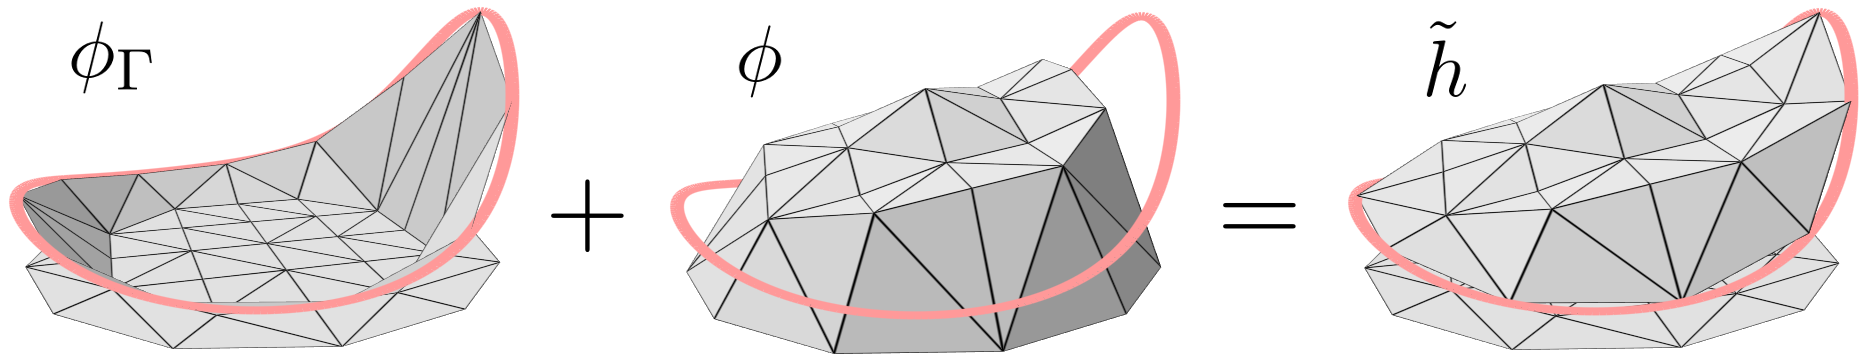
\includegraphics[width=1\linewidth]{figures/laplaceboundary/laplaceboundaryv2.png}
    \end{center}
    \caption{\scriptsize
        The fixed boundary approximation $\phi_\Gamma$ is added to a variable interior variation $\phi$ to give a possible approximate solution $\tilde{h}$.
        This possible solution can be checked by integration against the trial control volumes $\Omega_1,\cdots,\Omega_n$.
    }
    \label{laplaceboundary}
\end{figure}
\subsubsection{Choosing a finite number of control volumes}
If we choose some characteristic ``triangle centre'' for each triangle, then we can associate to the interior vertices
$p_1,\cdots,p_n$ a set of domains $\Omega_1,\cdots,\Omega_n$. Each $\Omega_i$ is determined by the polygon which joins the centres of the triangles
incident to $p_i$.
Two common choices for the triangle centre are the barycentre, which is the average position of the three vertices, and the circumcentre,
which is the centre of the unique circle passing through the three vertices. The circumcentre scheme gives what are called
``Voronoi cells'' due to their relation to Voronoi diagrams in computational geometry \cite{orourke}.
The resulting cell decompositions are displayed in figure
\ref{cell_decompositions}.

\begin{figure}[H]
    \begin{center}
        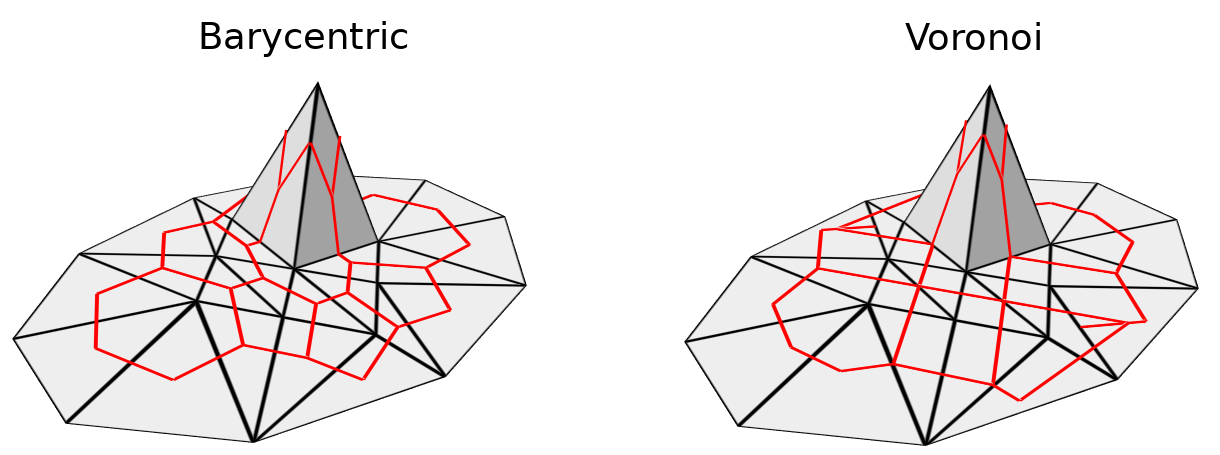
\includegraphics[width=0.7\linewidth]{figures/cell.png}
    \end{center}
    \caption{\scriptsize
        The domain $\Omega$ is partitioned into triangular cells $T_1\cdots T_{n_T}$.
        Flux integrals are taken over $n$ polygonal cells, one for each internal vertex $p_i$, for example using triangle barycenters or circumcentres.
        Notice that, in the circumcentre case, the thin triangles do not contain their circumcentre, and therefore each cell boundary is not necessarily
        contained in a single fan of triangles.
    }
    \label{cell_decompositions}
\end{figure}

The scheme as described so far, consisting of a triangle mesh, hat test functions, and barycentric or Voronoi control volumes,
has found some success, especially in the domain of geometry processing (\cite{polygon_mesh_processing}, \cite{ddg_triangulated}).
We will work with the Voronoi cells.

\subsubsection{Forming the linear system by closed-form integration}
Now that we have chosen a specific finite volume discretization, given a domain triangulation we can compute
the coefficients of the linear system \eqref{poisson_matrix_equation} and solve for $\hat{h}$, giving
the approximate solution $\tilde{h} = \phi_\Gamma + \Phi\cdot \hat{h}$.
By fortuitous circumstances, these integrals actually have simple closed forms, equivalent to geometric constructions.
Firstly, lets consider the trial flux integral
\begin{equation}\label{fvm_integral}
\int_{\pom_j} -\nabla \tilde{h}\cdot\hat{n}\,dx.
\end{equation}
By linearity, $\nabla \tilde{h}$ is a combination of gradients of basis functions of $\Phi^*$:
\begin{align*}
    \nabla \tilde{h} = \nabla\phi_\Gamma + \nabla\phi
             = \sum_{i=1}^{n_\Gamma}h_\Gamma(p^\Gamma_i)\nabla\phi^\Gamma_i + \sum_{i=1}^n h_i\nabla\phi_i.
\end{align*}
By linearity the integral \eqref{fvm_integral} becomes
\begin{equation}\label{fvm_integral_linearity_expanded}
    \sum_{i=1}^{n_\Gamma}\left[h_\Gamma(p^\Gamma_i)\int_{\Omega_j}-\nabla\phi^\Gamma_i\cdot\hat{n}\,dx\right]
    + \sum_{i=1}^n\left[h_i\int_{\Omega_j}-\nabla\phi_i\cdot\hat{n}\,dx\right].
\end{equation}

% We therefore need only compute the integrals
% $$
%     \int_{\Omega_j} \nabla\phi_i \cdot \hat{n}\,dx.
% $$
Let $v = p_j$ be the interior vertex corresponding to the control volume $\Omega_j$, and denote by $v_1, \cdots, v_k$ its adjacent vertices (either in the interior
or on the boundary), and by $T^v_1 \cdots T^v_k$ its adjacent triangles. Triangle $T^v_l$ joins $v,v_l,v_{l+1}$ where addition is taken
modulo $k$. As it will be necessary to relate these local indices to the global vertex indices, define an index map by
    $$I(v_i) = \text{the global index $l$ of the $p_l$ corresponding to adjacent vertex $v_i$},$$
which is valid only when $v_i$ is an interior vertex.
This vertex $v$ corresponds to a single trial flux integral over the surrounding Voronoi cell $\Omega_j$.
As the hat functions have compact support, $\Omega_j$ only intersects the domains of the basis function $\phi_j$ and those corresponding
to the adjacent vertices in the interior. Name these basis functions $\phi_j = \phi_v$ and $\phi_{v_1}, \cdots \phi_{v_k}$.
Then the integral becomes
\begin{equation}\label{fvm_integral_vertex}
    \int_{\Omega_j}-\nabla\phi_v\cdot\hat{n}\,dx + \sum_{i=1}^{k}h_{v_i}\int_{\Omega_j}-\nabla\phi^v_i\cdot\hat{n}\,dx,
\end{equation}
where $h_{v_i}$ is defined as
\begin{align*}
    h_{v_i} =
    \left\{\begin{array}{lr}
        h_\Gamma(p^\Gamma_i) &\text{if $v_i$ is a boundary vertex,}\\
        h_{I(v_i)} &\text{if $v_i$ is an interior vertex}.\\
        \end{array}\right.
\end{align*}
The $\phi_v$ and $\phi_{v_1},\cdots,\phi_{v_k}$ are hat functions which are linear when restricted to each triangle
$T^v_1,\cdots,T^v_k$. Therefore the gradients $\nabla\phi_v$ and $\nabla\phi_{v_1},\cdots,\nabla\phi_{v_k}$ are constant
on those triangles. We can break the closed flux integrals in \eqref{fvm_integral_vertex} into flux integrals restricted to each triangle adjacent to $v$, giving
\begin{equation}\label{fvm_integral_vertex_triangles}
    \sum_{t=1}^k\left[\int_{\Omega_j \cap T^v_t}-\nabla\phi_v\cdot\hat{n}\,dx + \sum_{i=1}^{k}h_{v_i}\int_{\Omega_j \cap T^v_t}-\nabla\phi^v_i\cdot\hat{n}\,dx\right].
\end{equation}
We now only need to find a closed form for
$$
\int_{\Omega_j \cap T_t^v} -\nabla\phi_v\cdot\hat{n}\,dx \text{\quad and \quad} 
\int_{\Omega_j \cap T_t^v} -\nabla\phi_{v_i}\cdot\hat{n}\,dx,
$$
which is simple because the gradients are constant on $\Omega_j \cap T_t^v$. We can simplify matters by focusing on just one adjacent triangle, say
$T = vv^\pr v^\ppr$

\vskip 0.2in
(figure)
\vskip 0.2in

The Voronoi polygon joins the midpoints $\frac{1}{2}(v + v^\pr)$ and $\frac{1}{2}(v + v^\ppr)$, taking a detour to the barycentre of $T$.
However, since the vector field $\nabla\phi_v$ is constant, it is conservative, and we can simplify the domain to the line segment $L$ between
the midpoints $\frac{1}{2}(v + v^\pr)$ and $\frac{1}{2}(v + v^\ppr)$.





% In geometry processing this matrix is called the ``cotangent Laplacian'' \cite{polygon_mesh_processing}, and it is typically
% applied to surface meshes in $\mathbb{R}^3$, which can be thought of as triangulations of a smooth surface.
% \subsection{Results and visualisation}
% \vskip 0.2in
% (results and visualisation)
% \vskip 0.2in
% We have worked through an instance of a \textit{finite volume method} \cite{pde_larsson}.
% Finite volume methods are characterised by a selection of a finite number of control volumes, and computation of flux integrals.
% Finite volume methods are typically \textit{conservative}, due to the ``flux network'' nature of the discretisation.

\section{From finite volumes to finite elements}\label{trial_function}
The alternative ``finite element'' approach is directly related to the ``finite volumes'' described above. While each finite volume
had a direct geometric meaning (as a small cell in which a certain test flux integral is taken), the geometric meaning of a ``finite element''
requires slightly more thought, although it will be seen to be the same idea in disguise.
The matrix equation \eqref{poisson_matrix_equation} consists of linear equations
\begin{align*}
    \int_{\pom_1} -\nabla \left(\sum_{i=1}^n h_i\phi_i\right) \cdot \hat{n}\,dx
    =
    \int_{\om_1}g\,dx\quad\text{(for $j=1$)},
\end{align*}
and so on. We cannot compute flux integrals
over all arbitrary control volumes, but we can take a number of ``trial'' flux integrals over the finite number of cells $\Omega_i$.
We can take linear combinations of these equations to get more equations which must hold on a solution.
For example,
\begin{equation}\label{example_trial_sum}
    \int_{\pom_1} -\nabla \left(\sum_{i=1}^n h_i\phi_i\right) \cdot \hat{n}\,dx
    +
    \int_{\pom_2} -\nabla \left(\sum_{i=1}^n h_i\phi_i\right) \cdot \hat{n}\,dx
    =
    \int_{\om_1}g\,dx
    +
    \int_{\om_2}g\,dx
\end{equation}
must hold. At first sight, \eqref{example_trial_sum} cannot directly be interpreted as a statement about a ``flux integral'', but rather about a sum
of flux integrals. However, a key idea is to regard \eqref{example_trial_sum} as a flux integral over a \textit{formal sum} of domains,
    $$\Omega_1 + \Omega_2.$$
We now have the equation
\begin{equation}
    \int_{\pom_1 + \pom_2} -\nabla \left(\sum_{i=1}^n h_i\phi_i\right) \cdot \hat{n}\,dx
    =
    \int_{\om_1 + \om_2}g\,dx.
\end{equation}
In differential geometry $\Omega_1 + \Omega_2$ is called a \textit{chain}. For example, we may visualise $\Omega_1 + 2\Omega_2 + 0.5\Omega_4$ as:

\vskip 0.2in
(draw this)
\vskip 0.2in

We define the boundary operator $\partial$ to be linear in formal sums e.g.,
    $$\partial(\Omega_1 + \Omega_2) = \pom_1 + \pom_2.$$
If $\om_1$ and $\om_2$ share a boundary, we would like $\om_1 + \om_2$ to represent their union, such that a flux
integral over $\partial(\Omega_1 + \Omega_2)$ evaluates to zero on the shared boundary. This can be done by thinking of
the boundary as \textit{oriented}, as in, consisting of oriented ``surface elements'' over which flux integrals can be taken.
For example, the $\hat{n}$ in a flux integral denotes the outward-pointing normal, which represents an ``outward-flux-measuring surface element''.
The opposite $-\hat{n}$ then represents the ``inward-flux-measuring surface element'', which is outward from the perspective of an adjacent cell.

\vskip 0.2in
(draw this)
\vskip 0.2in

We may now define
    $$\Psi = \text{span}\left\{\Omega_1,\cdots,\Omega_n\right\}$$
to be the \textit{trial space}, where the span is taken with respect to formal sums. As with a typical linear space,
we may choose from many possible bases. For example,
    $$\Psi = \text{span}\left\{\Omega_1, \Omega_2, \Omega_3\right\} =
    \text{span}\left\{\Omega_1 + \Omega_2, 2\Omega_2, \Omega_3\right\}.$$
A key idea, leading to Galerkin methods, is to allow freedom in the choice of the trial space $\Psi$.
Notably, we do not need $\Psi$ to be a space of formal sums of domains.
The Poisson equation is discretised over flux integrals around cell boundaries in the linear system \eqref{poisson_equation_integral_discretized},
which we repeat here:
\begin{align*}
    \sum_{i=1}^n h_i\int_{\pom_j} -\nabla \phi_i \cdot \hat{n}\,dx = \int_{\om_j} g\,dx,\quad j=1,\cdots,n.
\end{align*}
Applying Stokes' theorem, we get
\begin{align*}
    \sum_{i=1}^n h_i\int_{\om_j} -\Delta \phi_i \,dx = \int_{\om_j} g\,dx,\quad j=1,\cdots,n.
\end{align*}
We can think of these integrals as over the \textit{entire domain} $\Omega$, giving the form
\begin{align*}
    \sum_{i=1}^n h_i\int_{\om} -\Delta \phi_i\cdot \chi(\om_j)\,dx = \int_{\om} g\cdot\chi(\om_j)\,dx,\quad j=1,\cdots,n.
\end{align*}
where $\chi(\om_j)$ is the indicator function of $\om_j$,
\begin{align*}
    \chi(\om_j)(x) \coloneqq \left\{\begin{array}{lr}
        0 &\text{if $x \in \om_j$}\\
        1 &\text{if $x \notin \om_j$.}\\
        \end{array}\right.
\end{align*}
We can now think of our trial space $\Psi$ as a span of functions, instead of a span of domains:
    $$\Psi = \text{span}\left\{\chi(\Omega_1),\cdots,\chi(\Omega_n)\right\}.$$
Now, as the trial space is just a regular function space, we could instead let
    $$\Psi = \text{span}\left\{\psi_1,\cdots,\psi_n\right\}$$
where the $\psi_j$
need not be the indicator functions of a selection of control volumes. We now have the system of equations
\begin{align*}
    \sum_{i=1}^n h_i\int_{\om} -\Delta \phi_i \psi_j\,dx = \int_{\om} g\psi_j\,dx,\quad j=1,\cdots,n.
\end{align*}
By integration by parts we have the system of equations
\begin{equation}\label{poisson_galerkin}
    \sum_{i=1}^n h_i\int_{\om} \nabla \phi_i \cdot \nabla \psi_j\,dx = \int_{\om} g\psi_j\,dx,\quad j=1,\cdots,n,
\end{equation}
and we see that we still only require the $\phi_i$ to be in $H^1(\Omega)$.
We can see that equation \eqref{poisson_galerkin} is very similar to the exact fluxes in \eqref{poisson_equation_integral_discretized},
and indeed \eqref{poisson_galerkin} gives a discrete linear system in much the same way.
There is a real geometric sense in which \eqref{poisson_galerkin} is a ``blurred convolution'' of flux integrals.

--- Mention the weak form, the above is an alternative motivation using the discrete equations rather than
variational methods with the original PDE.

% \subsubsection{Integrating over trial functions versus integrating over domains}
% The above construction (generalising a finite-volume flux integral to a finite-element ``blurred flux'' integral) is further investigated
% below.
% We will work with the Dirac delta ``function'' (which is rather a distribution, or generalised function),
% defined by
% \begin{align*}
%     \int_{\omn} \delta_y\,dx = 
%     \left\{\begin{array}{lr}
%         1 &\text{if $y \in \omn$}\\
%         0 &\text{otherwise}.\\
%         \end{array}\right.
% \end{align*}
% For example, possibly under some regularity assumptions, we may represent a trial function $\psi_j$ on $\Omega$ as
%     $$f = \int_\Omega \delta_x f(x)\,dx,$$
% which could be called ``Riemann-integral-like''.
% We may instead represent $\psi_j$ in a ``Lebesgue-integral-like'' way by defining
%     $$L_y(\psi_j) \coloneqq \left\{z \in \Omega \mid \psi_j(z) = y\right\}$$
% to be a level set of $\psi_j$, the points of $\Omega$ for which $\psi_j = y$. We can then express $\psi_j$ as
%     $$\psi_j = \int_{-\infty}^\infty \left[\int_{L_y(\psi_j)} y\delta_x \,dx\right]\,dy.$$
% This gives $\psi_j$ as the totality of its level sets.
% For example, if we let $\Psi$ be spanned by the hat functions on some triangulation, each hat function $\psi_j$
% can be thought of as a totality of level sets culminating in the point-set of $\psi_j(p_j) = 1$.
% 
% \vskip 0.2in
% (draw this)
% \vskip 0.2in
% 
% The discretised Poisson equation \eqref{poisson_galerkin} involves an integral over $\nabla \phi_i \cdot \nabla \psi_j$,
% and we can compute this as
% \begin{equation}\label{flux_convolution}
% \begin{split}
%     \int_{\om} \nabla \phi_i \cdot \nabla \psi_j\,dx
%         &= \int_{-\infty}^\infty \int_{\om} \nabla\phi_i \cdot \nabla\left[\int_{L_y(\psi_j)} y\delta_z \,dz\right]\,dx\,dy\\
%         &= \int_{-\infty}^\infty y \int_{L_y(\psi_j)} \nabla\phi_i \cdot \hat{n}\,dx\,dy.
% \end{split}
% \end{equation}
% We have this final equality by noting that the gradient of $\psi_j$ at $x$, where $\psi_j(x) = y$, is orthogonal to the level set $L_y{(\psi_j)}$,
% and has length $y$:
% 
% \vskip 0.2in
% (draw this)
% \vskip 0.2in
% 
% We can think of the ``flux trial'' \eqref{poisson_galerkin} as involving ``blurred fluxes'' as in \eqref{flux_convolution}.
% For example, if we let $\Phi = \Psi$ be the set of hat functions on some triangulation
% of $\Omega$, then form and solve the matrix system, we get a generally non-conservative system of fluxes. We have lost conservativeness
% by the ``blurring'' of the flux integrals, but we may have gained advantages in terms of stability and convergence: in this case,
% the linear system will be symmetric-positive-definite, and stably solvable by, for example, conjugate gradients.

\section{Discretizing Poisson's equation by finite elements}

Equation \eqref{poisson_galerkin} gives a discrete linear system
\renewcommand{\integralentry}[2]{\int_{\Omega}\nabla\phi_{#2} \cdot \nabla\psi_{#1}\,dx}
\begin{equation}\label{poisson_fem_matrix_equation}
    A\hat{h} = \begin{bmatrix}
            \integralentry{1}{1} & \cdots & \integralentry{1}{n} \\
            \vdots & & \vdots \\
            \integralentry{n}{1} & \cdots & \integralentry{n}{n}
            \end{bmatrix}
    \begin{bmatrix} h_1 \\ h_2 \\ \vdots \\ h_{n-1} \\ h_n \end{bmatrix}
    =
    \begin{bmatrix} \int_{\om}g\psi_1\,dx \\ \int_{\om}g\psi_2\,dx \\ \vdots \\ \int_{\om}g\psi_{n-1}\,dx \\ \int_{\om}g\psi_{n}\,dx \end{bmatrix}
    = \hat{g}.
\end{equation}
This has quite a similar form to \eqref{poisson_matrix_equation}, but with boundary and cell integrals replaced by integrals over the entire
domain.
Again, if the control volumes $\Omega_1,\cdots,\Omega_n$ and test space $\Phi = \text{span}\left\{\phi_1,\cdots,\phi_n\right\}$
are chosen well, this linear system will be non-singular and hopefully well-conditioned.

\subsection{Choosing a test and a trial space}
Notice that the integrals in \eqref{poisson_fem_matrix_equation}, in contrast to \eqref{poisson_matrix_equation},
are over the \textit{entire domain}. It may be very costly in general to construct such a matrix, requiring
the computation of many large integrals. The finite element method, in particular, solves this problem
by ``localising'' basis functions of the test and trial spaces. Each basis test function $\phi_i$
has \textit{compact support}, meaning that there is some compact subdomain $D^\phi_i$ such that
\begin{align*}
    \phi_i(x) =
    \left\{\begin{array}{lr}
        \phi_i(x) &\text{if $x \in D^\phi_i$}\\
        0 &\text{otherwise},\\
    \end{array}\right.
\end{align*}
and similarly each basis trial function $\psi_i$ has some corresponding compact subdomain $D^\psi_i$ such that
\begin{align*}
    \psi_i(x) =
    \left\{\begin{array}{lr}
        \psi_i(x) &\text{if $x \in D^\psi_i$}\\
        0 &\text{otherwise}.\\
    \end{array}\right.
\end{align*}
This has the effect of reducing the domain of each integral in \eqref{poisson_fem_matrix_equation}, as
    $$\int_\Omega \nabla\phi_i \cdot \nabla\psi_j\,dx = \int_{D_i^\phi \cap D_j^\psi} \nabla\phi_i \cdot \nabla\psi_j\,dx. $$
With well-localised basis functions, the intersection will be
    $$D_i^\phi \cap D_j^\psi = \emptyset$$
for most indices $i,j$, implying the matrix \eqref{poisson_fem_matrix_equation} will be \textit{sparse}. In practice this allows
the use of iterative or graph-based sparse matrix algorithms which can be hugely more efficient than dense matrix computations of the same size.
The size of the matrix will increase quadratically with the number of nodes in the discretization, while the number of nonzeros
typically increases linearly.
A typical sparsity pattern for a finite element problem is shown in figure \ref{sparsity_pattern}.

\begin{figure}[H]
    \begin{center}
        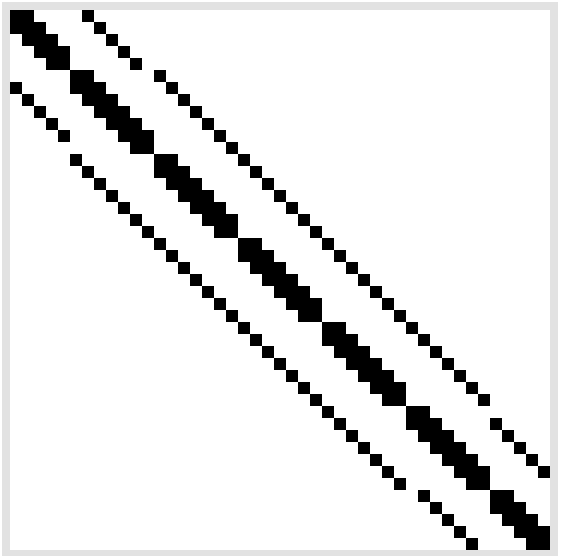
\includegraphics[width=0.26\linewidth]{figures/sparsity_pattern_no_text.png}
    \end{center}
    \caption{\scriptsize
        An example sparsity pattern for the finite element matrix of a 2D Poisson problem. White is zero and black is non-zero.
        The mesh has 61 vertices (16 on the boundary), and 104 triangles, resulting in a 45x45 system with 2025 entries, 197 non-zeros, and fill of $0.0973$.
    }
    \label{sparsity_pattern}
\end{figure}


Similar to the hat-functions-and-Voronoi-cells decomposition described for finite volumes,
the simplest scheme for the finite element Poisson equation is to triangulate $\Omega$ as
    $\bigcup_i T_i$
such there are $n$ nodal points and $n_T$ triangles.
Each nodal point $p_i$ will be associated with a piecewise linear ``hat'' basis function $\phi_i$ which is $1$ at $p_i$ and
$0$ at its neighbours. Now, diverging from the previous finite volume method, the simplest thing we could do is let the trial functions be the same
as the test functions, $\psi_i = \phi_i$. This trivially gives a one-to-one correspondence between the $\phi_i$ and the $\psi_i$, which will lead
to a well-formed linear system.

\vskip 0.1in
(draw this)
\vskip 0.1in

% It is at this stage that, in a finite volume method, we would choose a test space and a cell decomposition in one-to-one correspondence
% with a basis of the test space.
% In that case,
% there was the obvious candidate of a polygonal cell per-vertex.
% However, there is a vast array of possible Galerkin ``decompositions'' of the domain.
% A ``finite element method'', in particular, uses test and trial basis functions of \textit{compact support}.

We have so far worked up to an instance of a \textit{finite element method}.
Finite element methods are characterised by a test space $\Phi$ and trial space
$\Psi$ with basis functions of \textit{compact support}, where $\Phi$ and $\Psi$ typically consist of continuous functions in
some Sobolev space, constructed over a domain tessellation.

\section{Implementing the finite element method for Poisson's equation}
We now have an effective algorithm for approximating Poisson's equation:
\begin{enumerate}
    \item Partition the 2D domain $\Omega$ into triangles $T_i$. This implicitly defines the hat basis functions $\phi_i = \psi_i$.
    \item Form the matrix and right-hand-side in \eqref{poisson_fem_matrix_equation}, by analytical or numerical integration.
    \item Solve the resulting linear system for $\hat{h}$, and construct the solution as $\Phi\cdot\hat{h}$.
\end{enumerate}
Each of these steps is conceptually well-separated into the domains of
mesh generation, matrix assembly, and numerical linear algebra.

\subsection{Mesh generation}
Mesh generation is itself a huge field. However, there are only two essentials for the handling of 2D meshes and piecewise linear finite elements
--- a mesh data structure and a triangulator. Typically a mesh data structure will be provided by a separate library,
and the data organization (e.g., vertex, triangle, and adjacency information) will be designed to facilitate the kinds
of mesh traversals performed during matrix assembly. This is typically some variant of a ``halfedge'' data structure \cite{polygon_mesh_processing},
implemented in libraries such as Geometry Central \cite{geometry_central},
the Polygon Mesh Processing library \cite{polygon_mesh_processing_library}, and OpenMesh \cite{openmesh}.
A mesh data structure is a foundational component of \textit{mesh generation} systems. For 2D domains, a somewhat regular sampling of points on the boundary
and interior, followed by triangulation of these points, can suffice for a piecewise-linear finite element mesh.
The Triangle \cite{triangle} library, for example, contains a single very efficient and robust C routine (consisting of 16k lines of highly optimized code)
for performing Delaunay triangulations \cite{orourke}
on 2D domains,
with the specific goal of creating robust finite element meshes.


\subsection{Matrix assembly}
The matrix assembly stage is the core of a finite element implementation. The simplest idea is to iterate over all pairs $\phi_i$ and $\psi_j$,
letting $i=1,\cdots,n$, $j = 1,\cdots,n$, and approximate the integral $\int_\Omega \nabla\phi_i\cdot \nabla\cdot \psi_j\,dx$,
and store the value as entry $(i,j)$ of the matrix.
\begin{algorithm}
    \SetAlgoLined
    % \KwData{this text}
    % \KwResult{HOW}
    % initialization\;
    $M \leftarrow \text{zero matrix}$\;
    \For{$i=1,\cdots,n$}{
        \For{$j=1,\cdots,n$}{
            $M[i,j] \leftarrow \int_\Omega \nabla\phi_i\cdot \nabla\cdot \psi_j\,dx.$
        }
    }
\end{algorithm}

\begin{algorithm}
    % rhs computation
    \SetAlgoLined
    \For{$i=1,\cdots,n$}{
        $A \leftarrow 0$ \tcc*[l]{For computing total adjacent triangle areas.}
        \For{each triangle $T_j$ adjacent to $p_i$}{
            $A \leftarrow A + \text{Area}(T_j)$\;
        }
        $c \leftarrow g(p_i)$ \tcc*[l]{The source function is evaluated at the point $p_i$.}
        $\hat{b}[i] \leftarrow A\cdot c/3$\;
    }
\end{algorithm}

\begin{algorithm}
    % stiffness matrix computation and RHS boundary conditions.
    \SetAlgoLined

    $\text{Coefficients} \leftarrow \{\}$\;\tcc*[l]{This will contain triples $(i,j,\text{value})$ used to create the sparse matrix.}

    \For{each triangle $T_k$ in the domain partition}{
        $A \leftarrow \text{Area}(T_k)$\;
        $P,Q,R \coloneqq \text{The vertices of $T_k$}$\;
        $J \leftarrow \begin{bmatrix} Q_x-P_x & R_x-P_x \\ Q_y-P_y & R_y - P_y \end{bmatrix}$ \tcc*[l]{Jacobian of the reference transform.}
        $\text{Gradients} \leftarrow \left\{\begin{bmatrix} -1 & -1 \end{bmatrix},
                                            \begin{bmatrix} 1 & 0 \end{bmatrix},
                                            \begin{bmatrix} 0 & 1 \end{bmatrix}\right\}$\;
        $L \leftarrow \text{zero matrix}$ \tcc*[l]{The local stiffness matrix.}
        \For{$l,m=1,\cdots,3$}{
	    $L[l,m] \leftarrow A\left(\text{Gradients}[l] J^{-1}\right)\cdot\left(\text{Gradients}[m]J^{-1}\right)$\;
        }
        \For{$l,m=1,\cdots,3$}{
            \If{$p_{I(l)}$ is on the boundary}{skip\;}
            \If{$p_{I(m)}$ is on the boundary}{
                $\hat{b}[I(l)] \leftarrow \hat{b}[I(l)] - u_\Gamma(p_{I(m)})L(l, m)$\;
            }
            \Else{
                $\text{Coefficients} \leftarrow \text{Coefficients} \cup \left\{(I(l),I(m),L(l,m))\right\}$\;
            }
        }
    }
\end{algorithm}
    %     for (int i = 0; i < 3; i++) {
    %         for (int j = 0; j < 3; j++) {
    %             bool b1 = verts[i].on_boundary();
    %             bool b2 = verts[j].on_boundary();
    %             if (b1) {
    %                 continue; // The trial function can't be centered on the boundary.
    %             } else if (b2) {
    %                 auto p = geom.position[verts[j]];
    %                 double boundary_val = dirichlet_boundary_function(p.x(), p.z());
    %                 rhs[vertex_indices[verts[i]]] -= boundary_val*local_stiffness_matrix(i,j);
    %             } else {
    %                 coefficients.push_back(EigenTriplet(vertex_indices[verts[i]], vertex_indices[verts[j]], local_stiffness_matrix(i,j)));
    %             }
    %         }
    %     }

    % for (auto tri : geom.mesh.faces()) {
    %     Vertex verts[3];
    %     int vertex_index = 0;
    %     auto he = tri.halfedge();
    %     do {
    %         he = he.next();
    %         verts[vertex_index] = he.vertex();
    %     } while (++vertex_index < 3);

    %     auto A = geom.position[verts[0]];
    %     auto B = geom.position[verts[1]];
    %     auto C = geom.position[verts[2]];
    %     double triangle_area = 0.5*(B-A).cross(C-A).norm();

    %     // Compute the local stiffness matrix.
    %     Eigen::Matrix<double, 2,2> jacobian_matrix;
    %     jacobian_matrix <<
    %         B.x() - A.x(),  C.x() - A.x(),
    %         B.z() - A.z(),  C.z() - A.z();
    %     auto grad_transform = jacobian_matrix.inverse().transpose();
    %     Eigen::Matrix<double, 3,2> gradients;
    %     gradients <<
    %         -1,-1,
    %         1,0,
    %         0,1;
    %     Eigen::Matrix<double, 3,3> local_stiffness_matrix;
    %     for (int i = 0; i < 3; i++) {
    %         auto grad_i = grad_transform * gradients.row(i).transpose();
    %         for (int j = 0; j < 3; j++) {
    %             auto grad_j = grad_transform * gradients.row(j).transpose();
    %             local_stiffness_matrix(i,j) = triangle_area * grad_i.dot(grad_j); //*triangle_area ??????????????????????????????????????
    %         }
    %     }

    %     
    %     // Eigen::Matrix<double, 3,3> local_stiffness_matrix;
    %     // local_stiffness_matrix << 
    %     //     1, -0.5, -0.5,
    %     //     -0.5, 0.5, 0,
    %     //     -0.5, 0, 0.5;
    %     // local_stiffness_matrix *= 2*triangle_area;

    %     // i: Row, trial function.
    %     // j: Column, test function.

    %     for (int i = 0; i < 3; i++) {
    %         for (int j = 0; j < 3; j++) {
    %             bool b1 = verts[i].on_boundary();
    %             bool b2 = verts[j].on_boundary();
    %             if (b1) {
    %                 continue; // The trial function can't be centered on the boundary.
    %             } else if (b2) {
    %                 auto p = geom.position[verts[j]];
    %                 double boundary_val = dirichlet_boundary_function(p.x(), p.z());
    %                 rhs[vertex_indices[verts[i]]] -= boundary_val*local_stiffness_matrix(i,j);
    %             } else {
    %                 coefficients.push_back(EigenTriplet(vertex_indices[verts[i]], vertex_indices[verts[j]], local_stiffness_matrix(i,j)));
    %             }
    %         }
    %     }

    %     // std::cout << local_stiffness_matrix << "\n";
    %     // for (int i = 0; i < 3; i++) std::cout << (verts[i].on_boundary() ? "b " : "_ ");
    %     // std::cout << "\n";
    %     // std::cout << rhs << "\n";
    %     // getchar();
    % }

\subsection{Numerical linear algebra}
The solution of large linear systems is a vast topic in itself. Finite element solvers are typically clients
of standard, robust linear and non-linear solver libraries, such as Argonne National Laboratory's PETSc libraries \cite{petsc}
and the smaller-scale C\texttt{++} libraries Armadillo \cite{armadillo} and Eigen \cite{eigen}.
A finite element solver will typically pass either a full matrix to the linear solver (dense or sparse),
or provide the linear solver with callback routines that give the solver access to the system coefficients when they are needed.

\begin{figure}[H]
    \begin{center}
        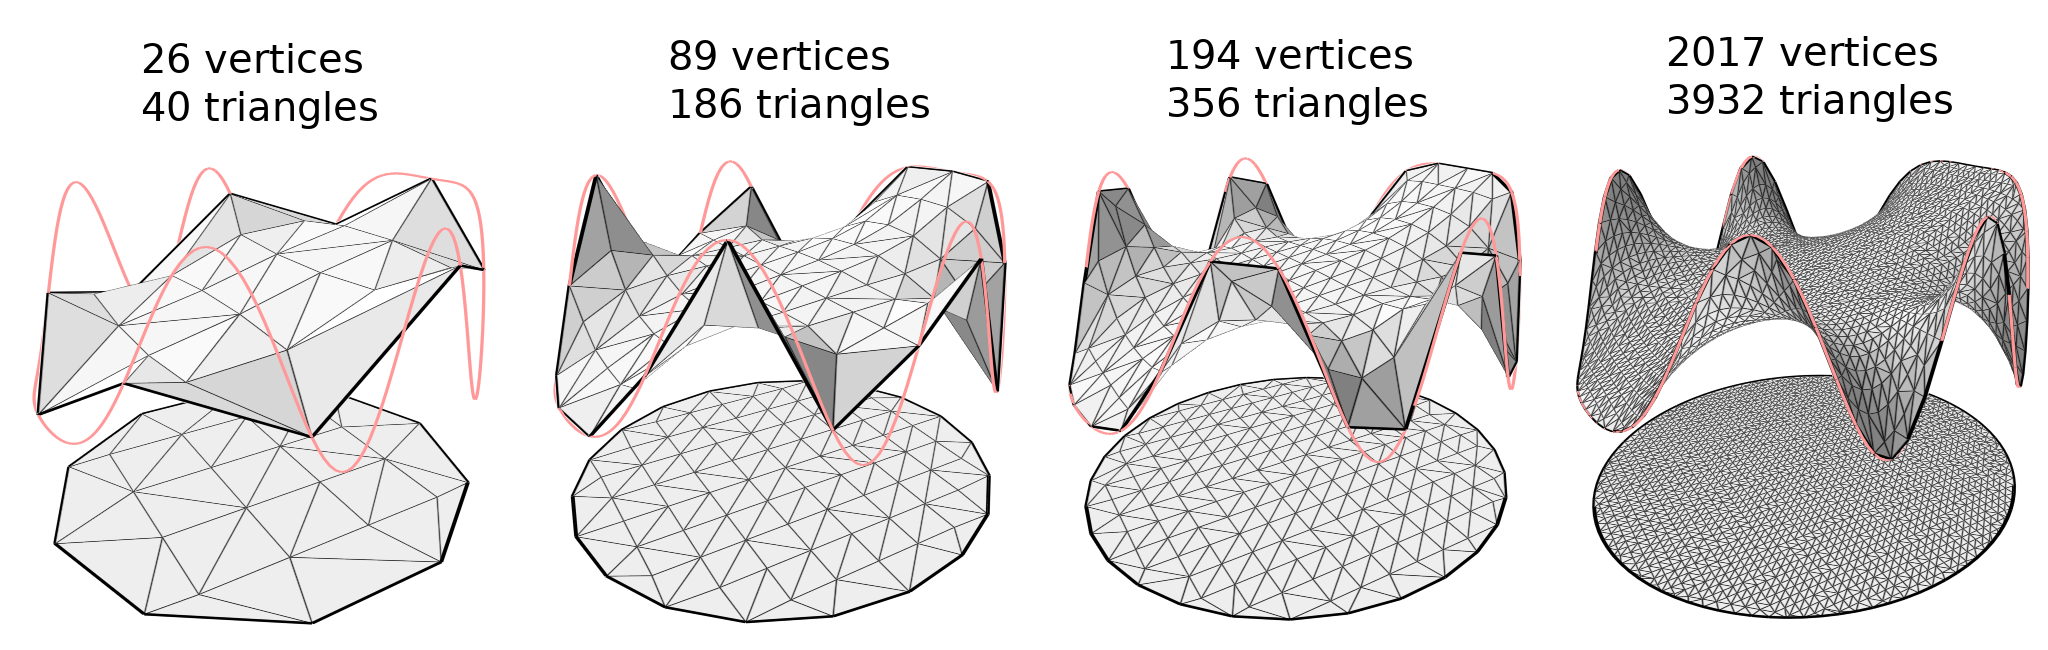
\includegraphics[width=\linewidth]{figures/laplace/laplacev2.png}
    \end{center}
    \caption{\scriptsize
        Text
    }
    \label{laplace_solution}
\end{figure}


% $$
%     h_\Gamma
% $$
% $$
%     \phi_\Gamma \in \Phi^*
% $$
% $$
%     \Gamma
% $$
% $$
%     T_1,\cdots,T_{n_T}
% $$
% 
% $$
%     p_1
% $$
% $$
% p_2
% $$
% 
% $$
%     p^\Gamma_1
% $$
% $$
%  p^\Gamma_2
% $$
% $$
%  p^\Gamma_3
% $$
% $$
% \cdots
% $$
% $$
% p^\Gamma_{n_\Gamma}
% $$
% $$
%     + \quad =
% $$
% $$
%     \phi_\Gamma \quad \phi = h_1\phi_1 + \cdots + h_n\phi_n \quad \tilde{h}
% $$
